\documentclass[11pt,
			   %10pt, 
               %hyperref={colorlinks},
               aspectratio=169,
               hyperref={colorlinks}
               ]{beamer}
\usetheme{Singapore}
\usecolortheme[snowy, cautious]{owl}

\usepackage[utf8]{inputenc}
\usepackage[T1]{fontenc}
\usepackage[american]{babel}
\usepackage{graphicx}
\usepackage{hyperref}
\hypersetup{
    colorlinks=true,
    urlcolor=[rgb]{1,0,1},
    linkcolor=[rgb]{1,0,1}}

\usepackage[natbib=true,style=authoryear,backend=bibtex,useprefix=true]{biblatex}
\usepackage{listings}
\lstset{numbers=right, 
        numberstyle=\tiny, 
%        breaklines=true,
%        backgroundcolor=\color{light-gray},
        numbersep=5pt,
	xleftmargin=\parindent,
	xrightmargin=.25in} 

%\setbeamercolor*{bibliography entry title}{fg=black}
%\setbeamercolor*{bibliography entry location}{fg=black}
%\setbeamercolor*{bibliography entry note}{fg=black}
\definecolor{OwlGreen}{RGB}{75,0,130} % easier to see
\setbeamertemplate{bibliography item}{}
\setbeamerfont{caption}{size=\footnotesize}
\setbeamertemplate{frametitle continuation}{}
\setcounter{tocdepth}{1}
\renewcommand*{\bibfont}{\scriptsize}
\addbibresource{bibliography.bib}

\renewcommand*{\thefootnote}{\fnsymbol{footnote}}

%\author{\copyright\hspace{1pt}Ashrith Barthur\footnote{\tiny{This material is shared under a \href{https://creativecommons.org/licenses/by/4.0/deed.ast}{CC By 4.0 license} which allows for editing and redistribution, even for commercial purposes. However, any derivative work should attribute the author and H2O.AI.}}}
\author{Ashrith Barthur}
\title{Machine Learning for Network Security}
\subtitle{Building Machine Learning Models to Detect and Mitigate Distributed Denial of Service Attacks}
\logo{
\includegraphics[height=8pt]{img/h2o_logo.png}}
\institute{\href{https://www.h2o.ai}{H\textsubscript{2}O.ai}}
\date{\today}
\subject{Building Machine Learning Models to Detect and Mitigate Distributed Denial of Service Attacks}

\begin{document}
	
	\maketitle
	
	\begin{frame}
	
		\frametitle{Contents}
		
		\tableofcontents{}
		
	\end{frame}

%-------------------------------------------------------------------------------
%	\section{Overview}
%-------------------------------------------------------------------------------
	\begin{frame}
		\frametitle{Overview}

		This presentation introduces us to three topics. These topics are:
		\begin{enumerate}
                \item The 101 on Distributed Denial of Service Attack.
                \item Building a Machine Learning model to identify the attack. 
                \item Feature building for Identification
                \item Deployment Architecture
		\end{enumerate}
	\end{frame}

%-------------------------------------------------------------------------------
%	\subection{H2O.AI Overview Team}
%-------------------------------------------------------------------------------
	\begin{frame}
		\frametitle{H2O.AI Overview}
		\begin{figure}[htb]
			\begin{center}
				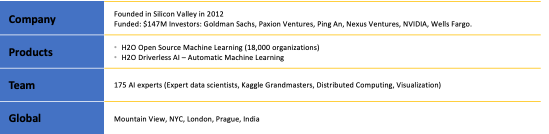
\includegraphics[width=0.95\textwidth]{img/team.png}
				\label{fig:team}
			\end{center}
		\end{figure}
	\end{frame}
%-------------------------------------------------------------------------------
%\subsection{H2O.AI Overview Areas}
%-------------------------------------------------------------------------------
	\begin{frame}
		\frametitle{Industry Footprint}
		\begin{figure}[htb]
			\begin{center}
				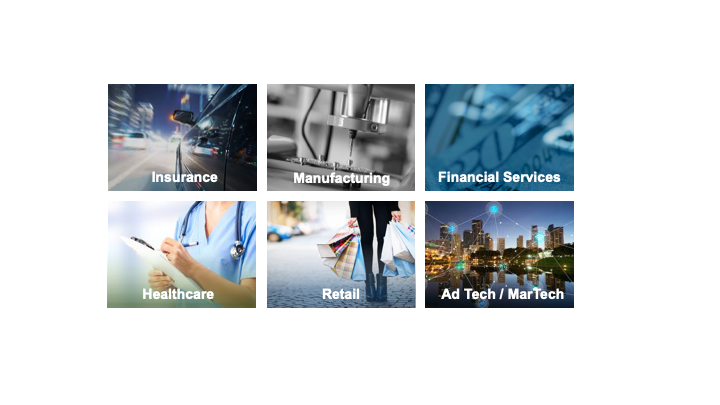
\includegraphics[width=0.95\textwidth]{img/industry.png}
				\label{fig:industry}
			\end{center}
		\end{figure}
	\end{frame}

%-------------------------------------------------------------------------------
%\section{DAI}
%-------------------------------------------------------------------------------
	\begin{frame}
		\frametitle{Driverless AI}
		\begin{figure}[htb]
			\begin{center}
				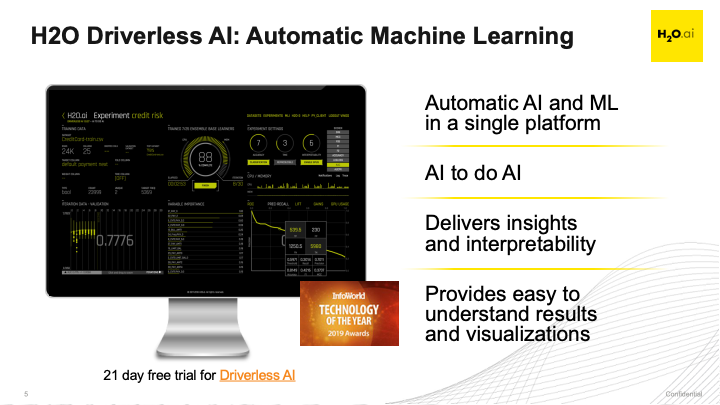
\includegraphics[width=0.75\textwidth]{img/dai.png}
				\label{fig:dai}
			\end{center}
		\end{figure}
	\end{frame}
%-------------------------------------------------------------------------------
%\section{DDoS}
%-------------------------------------------------------------------------------
%-------------------------------------------------------------------------------
	\subsection{DoS Introduction}
%-------------------------------------------------------------------------------
	\begin{frame}
		\frametitle{DoS}
        What is a DoS attack?\\
            \textit{A denial-of-service (DoS) attack occurs when a system floods the bandwidth or resources of a targeted system. Preventing or slowing the ability of the targeting system from further servicing any requests.}

	\end{frame}
%-------------------------------------------------------------------------------
%	\subsection{DDoS Introduction}
%-------------------------------------------------------------------------------
	\begin{frame}
		\frametitle{DDoS}
        What is a DDoS attack?\\
            \textit{"A distributed denial-of-service (DDoS) attack occurs when multiple systems flood the bandwidth or resources of a targeted system."}
	\end{frame}

%-------------------------------------------------------------------------------
%	\subsection{DDoS Current Design}
%-------------------------------------------------------------------------------
	\begin{frame}
            \frametitle{Current Detection}
		How are we detecting DDoS up until now?\\
		\begin{enumerate}
			\item We largely use Rule-Based systems and constant monitoring to identify potential DDoS traffic. 
            \item Much of this is depending on investigation, monitoring, filtering.
		\end{enumerate}

		Then what remains to be a problem?\\
		\begin{enumerate}
            \item A lot of these decisions are made after \textbf{traffic patterns are recognised, analysed, and modeled.} 
            \item This takes quite a bit of time causing large-scale systems and networks damage. 
			\item The Rules themselves are slow to identify new behaviour. 
		\end{enumerate}
	\end{frame}

%-------------------------------------------------------------------------------
%		\subsection{DDoS Recipe}
%-------------------------------------------------------------------------------
	\begin{frame}
            \frametitle{DDoS Data}

		\begin{enumerate}
                \item The data is an initial sliver of DDoS traffic that was captured. 
                \item The attack was targeting a \textit{http} server. 
		\end{enumerate}
	\end{frame}

%-------------------------------------------------------------------------------
%		\subsection{DDoS Recipe}
%-------------------------------------------------------------------------------
	\begin{frame}
            \frametitle{DDoS Data Transformations}

		\begin{enumerate}
                \item Building these transformations requires one to decide, if this is \textbf{analytical} or \textbf{production}.
                \item Analytical models are great for studying the behaviour and patterns, but could be slow when implemented. 
                \item Production models have simple traffic transformations but are quick. 
                \item By keeping the transformations simplistic, you keep pre-processing light, and allow the model to do the heavy lifting. 
		\end{enumerate}
	\end{frame}

%-------------------------------------------------------------------------------
%		\subsection{Question}
%-------------------------------------------------------------------------------
	\begin{frame}
		\frametitle{DEMO}
	\end{frame}

%-------------------------------------------------------------------------------
%	\subsection{Recipe Introduction}
%-------------------------------------------------------------------------------
	\begin{frame}[fragile]
		\frametitle{How Did We Build This?}
		Driverless AI provides an extension. \\
		This is a class `CustomTransformer`
		\begin{verbatim}
		class ExampleLogTransformer(CustomTransformer):
		\end{verbatim}
\end{frame}
%-------------------------------------------------------------------------------
%		\section{Feature Recipe Structure}
%-------------------------------------------------------------------------------
	\begin{frame}[fragile]
		\frametitle{How Did We Build This?}
		The class has:
		\begin{enumerate}
			\item Parameters that need to be provided. 
			\item These parameters are specific to the type of feature recipe that you are building. 
			\item It also has four methods which primary handle your feature engineering transformation. 
		\end{enumerate}
			
\end{frame}
%-------------------------------------------------------------------------------
%		\subsection{Parameters - Basic}
%-------------------------------------------------------------------------------
	\begin{frame}[fragile]
		\frametitle{Parameters - Basic}
		\begin{verbatim}
		class ExampleLogTransformer(CustomTransformer):
			_regression = True
			_binary = True
			_multiclass = True
		\end{verbatim}
			
\end{frame}
%-------------------------------------------------------------------------------
%		\subsection{Question}
%-------------------------------------------------------------------------------
	\begin{frame}
		\frametitle{Advantages}
		\begin{enumerate}
			\item Feature engineering process standardised by:
				\begin{enumerate}
					\item preset parameters
					\item preset methods
				\end{enumerate}
			\item Effort minimisation leads to minimisation in time spent.
			\item Build only once - Feature engineering is carried over from training/testing to production.
			\item DAI automatically, runs multiple models on various sets of features to get the best model. 
			\item All the requirements are handled internally by DAI. 
		\end{enumerate}
\end{frame}
%-------------------------------------------------------------------------------
%		\section{Feature Recipe Structure}
%-------------------------------------------------------------------------------
	\begin{frame}[fragile]
            \frametitle{Deployment Architecture}
		\begin{enumerate}
                \item Model is available as a Mojo - Java or C++, or as a Python Scorer. Depending on the infrastructure. 
                \item Model can score at a speed of 1.6M records per second. 
                \item Model is super-light, can be deployed at the edge node. 
                \item Model is independent, does not need help with decisions, (artifically intelligent)
                \item Can independently, stop malicious traffic in a shorter amount of time, much before its intercepted, analysed, and filtered. 
                \item Infrastructural damages can be prevented. Service availability is assured. 
		\end{enumerate}
			
\end{frame}
%-------------------------------------------------------------------------------
%	References
%-------------------------------------------------------------------------------

	\begin{frame}[t, allowframebreaks]
	
		\frametitle{References}	
		
			\textbf{How to build a recipe, Ashrith Barthur}\\
			\small{\url{https://github.com/h2oai/driverlessai-recipes/tree/master/how_to_write_a_recipe}}\\
            \textbf{A Streaming Statistical Algorithm for Detection of SSH Keystroke Packets in TCP Connections, DTIC}\\
            \small{Guha, Saptarshi ; Kidwell, Paul ; Barthur, Ashrith ; Cleveland, William S ; Gerth, John ; Bullard, Carter}\\
            \small{\url{https://apps.dtic.mil/dtic/tr/fulltext/u2/a534101.pdf}}\\
            \textbf{Toward Generating a New Intrusion Detection Dataset and Intrusion Traffic Characterization”, 4th International Conference on Information Systems Security and Privacy (ICISSP), Portugal, January 2018}\\
            \small{lIman Sharafaldin, Arash Habibi Lashkari, and Ali A. Ghorbani}\\

			
		\framebreak		
		
		\printbibliography
		
	\end{frame}
%-------------------------------------------------------------------------------
	\section{Questions}
%------------------------------------------------------------------------------

		\begin{frame}

                \frametitle{Thanks \& Questions}

		\end{frame}


\end{document}
\end{document}
